% This is samplepaper.tex, a sample chapter demonstrating the
% LLNCS macro package for Springer Computer Science proceedings;
% Version 2.20 of 2017/10/04
%
\documentclass[runningheads]{llncs}
%
\usepackage{graphicx}
% Used for displaying a sample figure. If possible, figure files should
% be included in EPS format.
\usepackage{color}
\usepackage{hyperref}
% If you use the hyperref package, please uncomment the following line
% to display URLs in blue roman font according to Springer's eBook style:
\renewcommand\UrlFont{\color{blue}\rmfamily}


\begin{document}
%
\title{Analysis of and Mitigation Strategies for \\Real World ICS Security Incidents}
%
%\titlerunning{Abbreviated paper title}
% If the paper title is too long for the running head, you can set
% an abbreviated paper title here
%
\author{Nico Fechtner}
%
\authorrunning{N. Fechtner}
% First names are abbreviated in the running head.
% If there are more than two authors, 'et al.' is used.
%
\institute{Technical University of Munich \& \\Fraunhofer Institute for Applied and Integrated Security\\
\href{mailto:nico.fechtner@tum.de}{nico.fechtner@tum.de}}
%
\maketitle              % typeset the header of the contribution
%
\begin{abstract}
% The abstract should briefly summarize the contents of the paper in
% 150--200 words.
% The goal is to communicate: Background/motivation/context, Aim/objective(s)/problem statement, Approach/method(s)/procedure(s), Results, Conclusion(s)/implications.
As more and more Industrial Control Systems (ICS) are getting connected to the internet and IT networks---intentionally or by mistake---the attack surface of these systems increases dramatically.
Due to this, the number of real world ICS security incidents rises, too, which is why it is crucial to develop efficient detection and mitigation strategies.
A solid baseline in this process is analyzing and learning from past incidents.
This is crucial to avoid common mistakes and to effectively prevent future incidents.
To aid this process, this paper proposes a systematic comparative overview of historic ICS security incidents focussing on various parameters including targets, threat actors, attack techniques, goals and impacts, dwell times, operator reactions and detection and mitigation strategies.
Several key findings are resulting from this overview and an in-depth analysis of the Triton incident.
First, x.
Second, y.
Third, z.

\keywords{ICS Security \and Security Incident \and Triton.}
\end{abstract}
%
%
%

\section{Introduction}
% The introduction supplies sufficient background information for the reader to understand and evaluate the work you did. Assume the reader is a generic computer science student, knowledgeable and acquainted with all basic computer science concepts. The introduction should also include a description of the problem you want to solve, your research questions, and an outline for the remainder of your paper. The goal is to: Indicate the field of the work, why this field is important, and what has already been done (with proper citations), Outline the purpose of your paper and announce your research questions, Avoid: repeating the abstract; providing unnecessary background information.
While Information Technology (IT) refers to software and hardware that generate data for enterprise use, Operational Technology (OT) describes software and hardware able to detect or cause a physical event in an industrial environment.
% ICS
Probably the most important subcategory of OT, at least revenue-wise, are Industrial Control Systems (ICS).
They are used in a wide variety of industries such as food and agriculture, energy, water, transportation, chemical, nuclear power, pharmaceutical and discrete manufacturing \cite{stouffer.2011}.\\
% OT Security <-> IT Security: very recent trend, first incidents
Initially, ICS were not connected to the internet and strictly separated from IT networks.
Due to this isolation, it was hard if not impossible for adversaries to remotely attack ICS which is why until recently security was not a big concern to companies running ICS.
Instead, they traditionally focus on safety, continuity and efficiency of their systems.
However, the attack surface of many ICS changed within the last two decades since they got connected to traditional IT networks and the internet---sometimes intentionally, sometimes by mistake.
Inevitably, this led to an ongoing series of ICS security incidents.\\
% Problem: No overview; Contribution: Overview
While more and more of those incidents are reported, it is business-critical to develop suitable detection and mitigation strategies.
A solid baseline in this process is analyzing and learning from past incidents.
This is crucial to avoid common mistakes and to effectively prevent future incidents.
To aid this process, this paper proposes a systematic comparative overview of historic ICS security incidents focussing on various parameters including targets, threat actors, attack techniques, goals and impacts, dwell times, operator reactions and detection and mitigation strategies.
% Benefits of an overview: Helps to identify patterns and to prevent future incidents (?)
The overview aims at identifying common attack patterns that could be used to prevent future attacks.
To the best of the author's knowledge, such an overview has not yet been published.\\
% Triton
In addition, the Triton incident of 2017 will be analyzed in detail to showcase how attackers perform sophisticated ICS attacks and which detection and mitigation strategies can be derived from their methodologies.
The incident was chosen due to its potential life-threatening impact and the novel attack approach targeting Safety Instrumented Systems (SIS).\\
% Outline
The remainder of the paper is structured as follows.
Section 2 provides an overview of related work in the area of ICS incidents which is used as the basis of the comparative overview that is provided in Section 3.
Exemplary the Triton incident is analyzed in detail in Section 4.
Section 5 concludes the paper by emphasizing the need to learn from past mistakes.
\section{Related Work}
% In this section, you provide an overview of papers written by other scientists that have covered a problem similar to yours. You can find related work in web search engines and scientific literature databases. Some of the most prominent ones in the field of computer science are: Google Scholar, Scopus, ACM Digital Library, IEEE Xplore, Lecture Notes in Computer Science.
There are four main types of publicly available sources that provide information on ICS security incidents.
% Enumerations: RISI Database, ICS-CERT Alerts from the US Government,
First, there are incident enumerations like the Risi Database\footnote{https://www.risidata.com/Database} and the ICS-CERT Alerts\footnote{https://www.us-cert.gov/ics/alerts}.
On the one hand, the fact that those repositories aim to aggregate all observed ICS incidents from around the world makes them useful for getting a high-level overview of the current threat landscape.
On the other hand, however, they only provide basic information about the incidents and do not analyze them in detail.
% Reports from Companies in the field: Dragos Threat Report, CyberX Global IoT/ICS Risk Report,...
Second, ICS security companies like Dragos \cite{dragos.19} and CyberX \cite{cyberx.19} publish yearly ICS threat reports discussing relevant incidents.
Those reports are neither complete with regards to the incidents they cover nor do they provide in-depth analyses of the covered attacks.
However, they do a good job of highlighting trends in the threat landscape throughout the years.
Third, dedicated scientific papers are focussing on single ICS incidents like the attacks targeting the Ukraine power grid \cite{eisac.16} or the Triton malware \cite{pinto.18}. Those papers usually cover single incidents in-depth and help in understanding how exactly the adversaries operated.
Fourth, there are numerous blog posts, press releases, and conference talks covering ICS incidents.
In addition, there is the MITRE ATT\&CK ICS database\footnote{https://collaborate.mitre.org/attackics/index.php/Main\_Page} which includes information on tactics, techniques, and software used by threat groups to perform ICS attacks.
Furthermore, there is a paper proposing an overview of historical ICS security incidents \cite{hemsley.18}.
However, it is slightly dated and, more importantly, does not compare the different incidents systematically.
All of the above-mentioned sources are taken into account to achieve exactly this in the upcoming section.

% Other papers covering the big incidents: Ukraine, Triton,...
% IT incidents overview
\section{Comparative Overview of ICS Security Incidents}
From the literature and resources stated in Section 2, a total of 29 ICS security incidents were extracted.
Those form the basis of the following analysis and can be found in table [appendix table].
Note that due to incidents not being reported, the tremendous amount of incidents that are reported and new incidents occurring steadily, this table is inherently incomplete, but rather tries to focus on the most prevalent attacks launched until February 2020.
In the subsections below, a comparative overview of these incidents will be given.
Each subsection tries to compare the incidents with regards to specific attributes, e.g. the involved threat actors or the utilized attack techniques.
% (
% Most subsections contain both quantitative as well as qualitative statements.
% Please keep in mind, though, that the quantitative numbers are solely intended to highlight important trends and that the according values might contains inaccuracies.
% This is due to the fact that often specific information about incidents is unknown or not known for sure.
% For example, consider the dwell time which describes how long an adversary is in a system before the actual attack payload is executed.
% Sometimes it is possible to give an accurate estimation for this number thanks to digital forensics after an incident.
% In general, however, this is a non-trivial task and even if performed successfully, it may still lead to incorrect conclusions about the dwell time and other incident attributes.
% )

\subsection{Targets}
% Targeted vs. Untargeted
When analyzing the entities affected by ICS security incidents there are two fundamentally different kinds of attacks that have to be considered separately.
On the one hand, there are targeted attacks against unique entities.
Making up roughly 86\% of the analyzed incidents, targeted attacks seem to present a diverse threat landscape to ICS and will therefore be analyzed in detail below.
On the other hand, there are untargeted attacks.
Here, the threat actors are not interested in the specific entities that will be affected by the attack, but rather they aim for as many incidents as possible.
Often this is achieved by a self-replicating component within the malware used for the attacks.
While only four of the analyzed incidents fall into this category, they still pose a significant threat to ICS.
Interesting to see is that the malware used for untargeted attacks usually is not tailored specifically for ICS environments, but rather targets common operating systems like Microsoft Windows and enterprise networks in general.
Many instances of untargeted attacks fall in the category of ransomware.
For example, the popular WannaCry ransomware spread not only to desktop computers around the world but also infected a series of ICS workstations e.g. at a Taiwanese manufacturing plant leading to outages due to encrypted hard drives \cite{skybox.18}.
This kind of incidental infections of ICS systems with malware originally intended for enterprise networks are becoming more and more of a threat in recent years \cite{dragos.19}, \cite{cyberx.19}, \cite{zimba.18}.\\
% Untargeted
Since untargeted attacks are not aimed at specific entities but often solely intend to infect as many systems as possible, e.g. with self-replicating components, there is in general no pattern observable in terms of the geographical location or the economic sector of the affected parties.
Targeted attacks, however, can be analyzed for such patterns.\\
% Country
When it comes to the geographical location of ICS attack victims, the areas most often affected seem to be the Middle East and Europe. The Middle East is being targeted by about 56\% of the analyzed attacks. Especially companies located in Saudi Arabia often fall victim to attacks. Probably the most well-known incident taking place there was Triton which targeted a Saudi Arabian petrochemical plant and will be covered in depth in Section 4.
Companies located in Europe are targeted by about 52\% of the analyzed attacks. The country affected the most until now is Ukraine falling victim to multiple attacks targeting its power grid.
In about 24\% of the analyzed incidents, the US were amongst the victims.
Interesting is that while being home to important global threat actors as discussed in Subsection 3.2, neither Russia nor China nor North Korea reports a lot of ICS incidents against entities located in their countries.
However, this does not necessarily mean that no ICS incidents occur in these countries, but it could also be the case that incidents are just not as liberally published as by other countries.
Especially China and North Korea are known for withholding most of the cyber attacks taking place in their country [citation].\\
% Sector (+ private/public)
When it comes to the economic sector falling victim to targeted ICS attacks, the most affected one is the energy sector being targeted in about 52\% of the analyzed targeted attacks.
Most and foremost, those operations include attacks against power grids like the attacks taking place in 2014 and 2015 in Ukraine.
Other examples of targeted entities within the energy sector include oil and gas pipelines and refineries.
The remaining victims of ICS attacks are spread across a wide variety of other economic sectors including manufacturing, water, petrochemical, governmental organizations and transportation.

\subsection{Threat Actors}
% General
In total, 16 specific threat actors were involved in the analyzed ICS incidents according to the current state of research.
% (
Note, that there are often multiple names for a single threat group.
They originate from different ICS security agencies and companies \cite{thaicert.19} and can be used interchangeably.
This paper tries to use to the most commonly used names regardless of which entity coined it.\\
% )
% Problem of Attribution
When it comes to the threat actors responsible for ICS attacks there is the fundamental issue of attribution.
Most often, threat actors want to stay anonymous and do not confess performed attacks. % Counterexample?
Therefore, there are often only conjectures about the threat actors involved in certain attacks.
In line with that, 38\% of the analyzed attacks cannot be associated with a specific threat actor.
% Where are Threat actors located?
Furthermore, it is often difficult to locate threat actors geographically, since they usually apply various techniques to hide their physical location \cite{huang.18}.
With regards to the analyzed incidents, 38\% of the threat groups cannot be associated with a specific country.
It can be said, however, that 28\% of all analyzed attacks are known to originate from Russia and 24\% are known to originate from the Middle East, thereof 71\% from Iran.
Other countries being home to important threat groups are China, the US and North Korea.
% Which are the most important threat actors?
The most active threat actors according to the sample of incidents taken into account here, are Energetic Bear from Russia, being involved in 14\% of all attacks, and APT33 from Iran, being involved in 10\% of all attacks.
% Collaboration
Interesting to note is, that some threat groups primarily act on their own while others collaborate with each other.
For example, APT33 often collaborates with other Iranian threat groups, whereas Energetic Bear mostly acts alone.
% Team Size
When it comes to the team size, only one threat actor is an individual person, all others are groups comprised of multiple people.
This person, Vitak Boden, performed what can be considered one of the first ICS attacks ever.
To take revenge on a wastewater facility where he was rejected when applying for a job, he manipulated the sewage pumping stations via an RF transmitter which lead to millions of gallons of untreated sewage water being released into waterways and local parks \cite{hemsley.18}.
Since this incident in the year 2000, ICS attacks got a lot more sophisticated which is why the team size of threat groups continues to grow.\\
% Who is behind threat groups? Nation State Actors?
72\% of the analyzed attacks are considered to be performed by government-funded threat actors.
On the one hand, targeted ICS attacks require a large amount of knowledge and resources which often only nation-states can provide.
On the other hand, governments can profit in various ways from ICS attacks against foreign countries, be it through industrial espionage, by making critical facilities and infrastructures unavailable or even by targetting human lives.
Often ICS attacks can be seen as an act of war. % Citations and further research.

\subsection{Attack Techniques}
% ICS cyber kill chain
An established model to characterize ICS attacks is the ICS Cyber Kill Chain developed by the SANS institute and depicted in figure \ref{fig:CyberKillChain}.
It is comprised of two stages.
In stage one, IT intrusion preparation and execution takes places, i.e. the attacker compromises the IT network and positions herself in the ICS network.
This stage can be completed without specific knowledge about ICS technologies or protocols.
In stage two, ICS attack development and execution are performed, e.g. an attack targetting certain actuators---for example, water pumps---is developed, tested, and executed.\\
% Stage 1: Intrusion
When it comes to the initial access in stage one of the ICS Cyber Kill Chain, two attack techniques seem to be most popular among the analyzed incidents.
The first one is spearphishing which was reportedly performed in at least 26\% of the attacks.
The second one are zero day exploits which were utilized in at least 11\% of the attacks.
When inside the victims IT network, attackers often use common software.
For example, in at least 11\% of the cases Mimikatz was used for credential capturing.
Often, popular exploitation frameworks like Metasploit and Cobalt Strike are used, too.
More recent trends are the use of sophisticated obfuscation and evasion techniques and \textit{living off the land} tools---like PowerShell or PsExec---in order to avoid being detected by IDS.\\
% Untargeted Attacks
Since the core of untargeted attacks is usually ransom- or wiperware, they do not go beyond stage one of the ICS Cyber Kill Chain.
% Targeted Attacks
Targeted attacks, however, aim more and more often to exploit the ICS environment, which requires the attackers to first gain access to the ICS network.
One possible way to pivot is lateral movement via Windows authentication services.
% Stage 2: ICS Attack
Once in the ICS network, a multitude of different exploit strategies has been reported.
Most adversaries attack ICS components like Programmable Logic Controllers (PLCs) or Safety Instrumented Systems (SIS) to modify their behaviour or to make them fail altogether.
Doing so, they are often able to control actuators like waterpumps, fake the values of sensors or turn off the power supply.
To make disaster recovery harder, attackers often wipe Human-Machine Interfaces (HMIs), too.
% Special Case: Target Store's HVAC
While according to the ICS Cyber Kill Chain stage one typically has to take place before stage two, there is an example where the attack was performed the other way around.
In 2013, an unknown attacker stole login credentials of a third-party heating, ventilation, and air conditioning (HVAC) contractor of US Target Stores.
From the ICS network she then pivoted into the IT network in order to install credit card stealing software. \cite{hemsley.18}\\
% Scalability of the attack: Trend goes to scalable frameworks?
One important trend in addition to the techniques described above is the trend away from highly manual attacks specifically tailored for a single victim towards more victim-agnostic ICS attack frameworks enabling scalable attacks.
A case in point are the attacks on the Ukraine power grid.
The first attack in 2015 was highly manual and the effort put into it could not be directly utilized for attacks against other energy infrastructures.
One year later, however, there was a second attack targeting the power grid, but this time the adversaries had developed a framework which in theory allows them to scale their attack to a multitude of different victims with a relatively small effort. \cite{greenberg.17}
\begin{figure}[h]
    \fbox{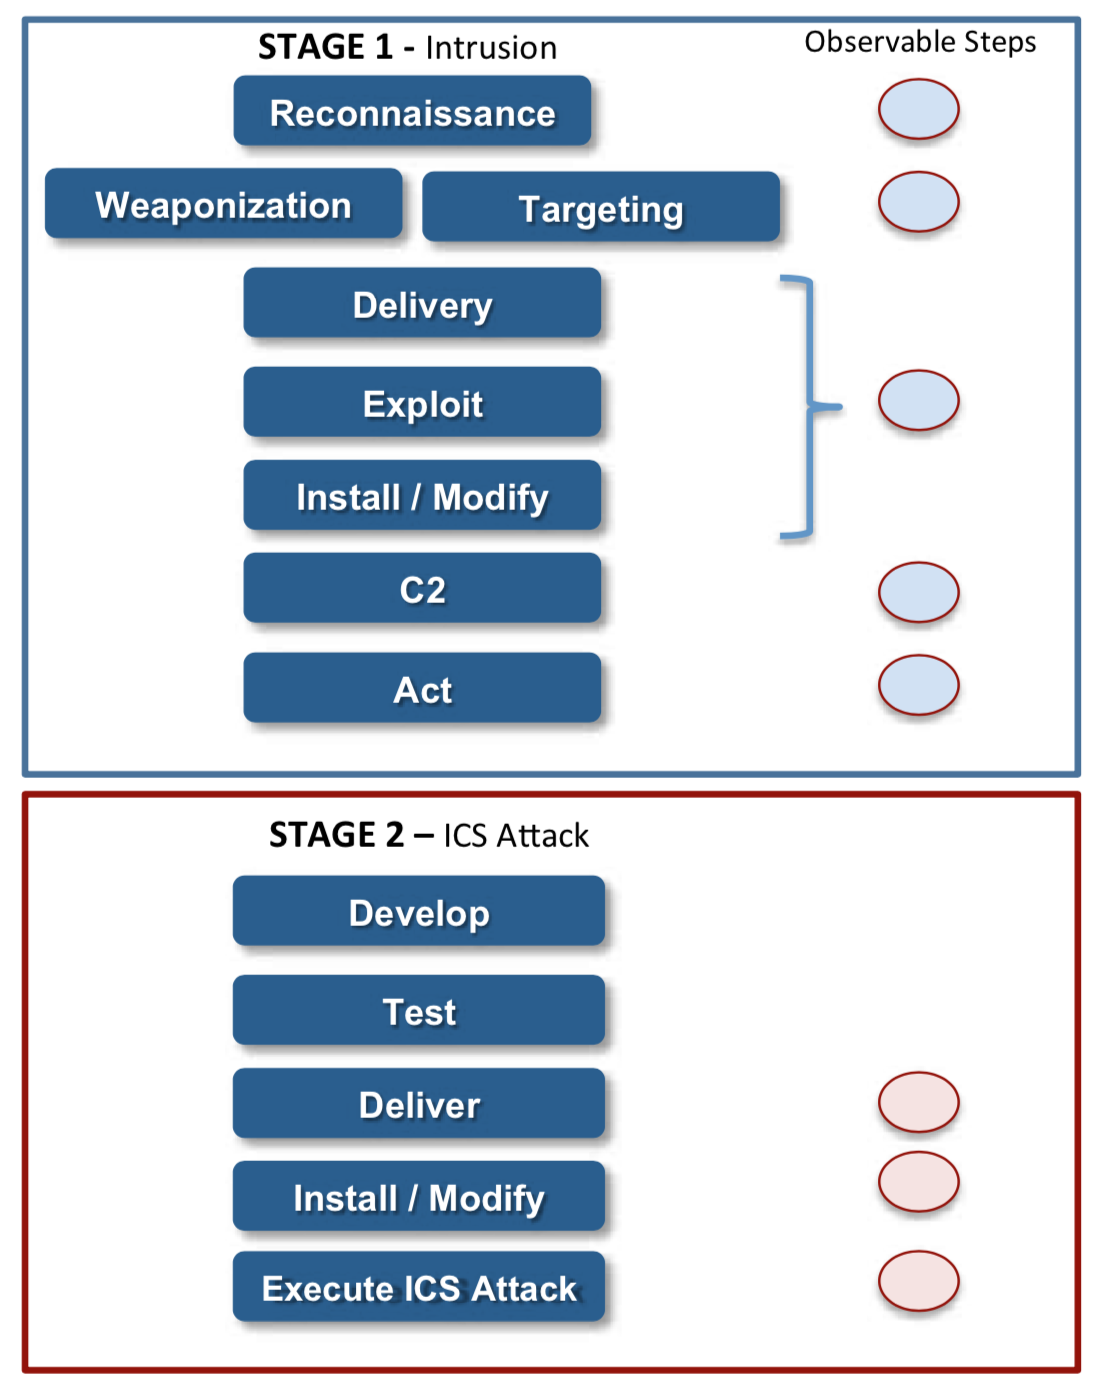
\includegraphics[width=\textwidth]{figures/ICSCyberKillChain.png}}
    \caption{ICS Cyber Kill Chain as introduced by the SANS institute, from \cite{assante.15}.}
    \label{fig:CyberKillChain}
\end{figure}
\subsection{Attack Goals and Realized Impacts}
% Common goals
The most common goal of adversaries is to extract data from the victim's systems. 37\% of all analyzed attacks were designed to achieve exactly this.
Other goals often persued by attackers are to cause disruption (22\%), to provoke a ransom payment (15\%), and to cause physical damage (11\%).\\
% Underlying motivations (state actors)
When it comes to the underlying motivations of attackers, three distinct ones seem to dominate.
First, attackers often strive for monetary gain.
This motivates ransomware attacks like WannaCry or LockerGoga as well as information stealing with the goal of selling the data to the highest bidder.
Second, some adversaries are interested in the data they steal themselfs and do not intend to sell them.
This motivates ICS espionage operations like StoneDrill were Iranian threat groups gathered intelligence about Saudi Arabian ICS environments.
Third, there are threat actors which intend to disrupt the regular operation of ICS by causing outages or even physical damage.
The latter was e.g. the case in the famous Stuxnet incident in 2010 were the US and Israelian government attacked nuklear enrichment facilities of Iran in order to sabotage the possible development of nuklear weapons.
Untargeted attacks falling into this category are typically related to wiperware which erases or encrypts hard drives without a subsequent ransom demand.\\
% How often were they successful
In total, a minimum of 85\% of the attacks are considered to be at least partly successful in achieving their goals with regards to some of their victims.
% Impacts, when successful
Typical impacts include information loss, financial loss---via physical damage, ransom payment or costly recovery processes---and environmental damages.
Fortunately, until to date, there are no ICS incidents known which killed humans.\\
% If not successful, why?
One incident considered to be unsuccessful is the well-known Triton attack which failed for reasons not fully understood up until today.
Section 4 will provide a detailed analysis of the incident and its impacts.
Furthermore, untargeted attacks often partly fail to achieve their goal since a lot of companies can restore operations without a long outage or paying a ransom thanks to sufficient backup strategies.
\subsection{Dwell Times and Reactions}
% Dwell times
% Time of Discovery
% Typical Reactions (do they help?)
\subsection{Detection and Mitigation Strategies}
% Mitigation against untargeted ransom- & wiperware
% Asset Inventory
% Vulnerability Management Software
% Anomaly/Incident Detection System
% Threat Hunting
% Security Awareness
% Firewalls
% Patching (hard)
% Network Segmentation (hard)

\section{Detailed Analysis of the Triton Attack}
\subsection{The Attackers' Approach}
\subsection{Impact}
\subsection{Attribution}
\subsection{Detection and Mitigation Opportunities}
% Asset Inventory
% Vulnerability Management Software
% Anomaly/Incident Detection System
% Threat Hunting
% Security Awareness
% Firewalls
% Patching (hard)
% Network Segmentation (hard)
\section{Conclusion}
% The conclusion summarizes the research and discusses its significance. You should also point out future research directions. The goal is to: Provide a very brief summary of the results, Provide a future perspective on the work, Avoid: repeating the abstract; repeating background information from the introduction; introducing new arguments; repeating the arguments made in the main body; failing to ad- dress all of the research questions set out in the introduction.
% Summary
% Learn from past mistakes
% Future Work

\newpage
%
% ---- Bibliography ----
%
% BibTeX users should specify bibliography style 'splncs04'.
% References will then be sorted and formatted in the correct style.
%
\bibliographystyle{splncs04}
\bibliography{bibliography}
\end{document}
